\documentclass{extbook}[14pt]
\usepackage{multicol, enumerate, enumitem, hyperref, color, soul, setspace, parskip, fancyhdr, amssymb, amsthm, amsmath, bbm, latexsym, units, mathtools}
\everymath{\displaystyle}
\usepackage[headsep=0.5cm,headheight=0cm, left=1 in,right= 1 in,top= 1 in,bottom= 1 in]{geometry}
\usepackage{dashrule}  % Package to use the command below to create lines between items
\newcommand{\litem}[1]{\item #1

\rule{\textwidth}{0.4pt}}
\pagestyle{fancy}
\lhead{}
\chead{Answer Key for Module7 Version A}
\rhead{}
\lfoot{4758-2646}
\cfoot{}
\rfoot{testing}
\begin{document}
\textbf{This key should allow you to understand why you choose the option you did (beyond just getting a question right or wrong). \href{https://xronos.clas.ufl.edu/mac1105spring2020/courseDescriptionAndMisc/Exams/LearningFromResults}{More instructions on how to use this key can be found here}.}

\textbf{If you have a suggestion to make the keys better, \href{https://forms.gle/CZkbZmPbC9XALEE88}{please fill out the short survey here}.}

\textit{Note: This key is auto-generated and may contain issues and/or errors. The keys are reviewed after each exam to ensure grading is done accurately. If there are issues (like duplicate options), they are noted in the offline gradebook. The keys are a work-in-progress to give students as many resources to improve as possible.}

\rule{\textwidth}{0.4pt}

\begin{enumerate}\litem{
Determine the domain of the function below.
\[ f(x) = \frac{6}{15x^{2} +15 x -30} \]The solution is \( \text{All Real numbers except } x = -2.000 \text{ and } x = 1.000. \), which is option D.\begin{enumerate}[label=\Alph*.]
\item \( \text{All Real numbers except } x = a \text{ and } x = b, \text{ where } a \in [-19, -15] \text{ and } b \in [24, 27] \)

All Real numbers except $x = -18.000$ and $x = 25.000$, which corresponds to not factoring the denominator correctly.
\item \( \text{All Real numbers except } x = a, \text{ where } a \in [-4, 0] \)

All Real numbers except $x = -2.000$, which corresponds to removing only 1 value from the denominator.
\item \( \text{All Real numbers except } x = a, \text{ where } a \in [-19, -15] \)

All Real numbers except $x = -18.000$, which corresponds to removing a distractor value from the denominator.
\item \( \text{All Real numbers except } x = a \text{ and } x = b, \text{ where } a \in [-4, 0] \text{ and } b \in [1, 4] \)

All Real numbers except $x = -2.000$ and $x = 1.000$, which is the correct option.
\item \( \text{All Real numbers.} \)

This corresponds to thinking the denominator has complex roots or that rational functions have a domain of all Real numbers.
\end{enumerate}

\textbf{General Comment:} Recall that dividing by zero is not a real number. Therefore the domain is all real numbers \textbf{except} those that make the denominator 0.
}
\litem{
Determine the domain of the function below.
\[ f(x) = \frac{6}{20x^{2} +31 x + 12} \]The solution is \( \text{All Real numbers except } x = -0.800 \text{ and } x = -0.750. \), which is option C.\begin{enumerate}[label=\Alph*.]
\item \( \text{All Real numbers except } x = a \text{ and } x = b, \text{ where } a \in [-20.02, -19.99] \text{ and } b \in [-12.01, -11.97] \)

All Real numbers except $x = -20.000$ and $x = -12.000$, which corresponds to not factoring the denominator correctly.
\item \( \text{All Real numbers except } x = a, \text{ where } a \in [-20.02, -19.99] \)

All Real numbers except $x = -20.000$, which corresponds to removing a distractor value from the denominator.
\item \( \text{All Real numbers except } x = a \text{ and } x = b, \text{ where } a \in [-0.81, -0.77] \text{ and } b \in [-0.79, -0.7] \)

All Real numbers except $x = -0.800$ and $x = -0.750$, which is the correct option.
\item \( \text{All Real numbers except } x = a, \text{ where } a \in [-0.81, -0.77] \)

All Real numbers except $x = -0.800$, which corresponds to removing only 1 value from the denominator.
\item \( \text{All Real numbers.} \)

This corresponds to thinking the denominator has complex roots or that rational functions have a domain of all Real numbers.
\end{enumerate}

\textbf{General Comment:} Recall that dividing by zero is not a real number. Therefore the domain is all real numbers \textbf{except} those that make the denominator 0.
}
\litem{
Solve the rational equation below. Then, choose the interval(s) that the solution(s) belongs to.
\[ \frac{-7x}{2x -3} + \frac{-2x^{2}}{8x^{2} +2 x -21} = \frac{5}{4x + 7} \]The solution is \( \text{There are two solutions: } x = 0.228 \text{ and } x = -2.195 \), which is option B.\begin{enumerate}[label=\Alph*.]
\item \( x \in [-2.68,-1.86] \)


\item \( x_1 \in [-0.08, 0.28] \text{ and } x_2 \in [-4.5,1.2] \)

* $x = 0.228 \text{ and } x = -2.195$, which is the correct option.
\item \( \text{All solutions lead to invalid or complex values in the equation.} \)


\item \( x_1 \in [-0.08, 0.28] \text{ and } x_2 \in [1.3,4] \)


\item \( x \in [-1.96,-1.47] \)


\end{enumerate}

\textbf{General Comment:} Distractors are different based on the number of solutions. Remember that after solving, we need to make sure our solution does not make the original equation divide by zero!
}
\litem{
Choose the graph of the equation below.
\[ f(x) = \frac{1}{x - 3} - 2 \]The solution is the graph below, which is option E.
\begin{center}
    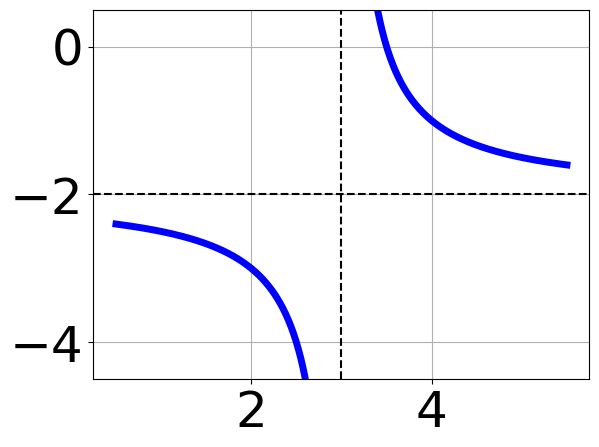
\includegraphics[width=0.3\textwidth]{../Figures/rationalEquationToGraphEA.png}
\end{center}\begin{enumerate}[label=\Alph*.]
\begin{multicols}{2}
\item 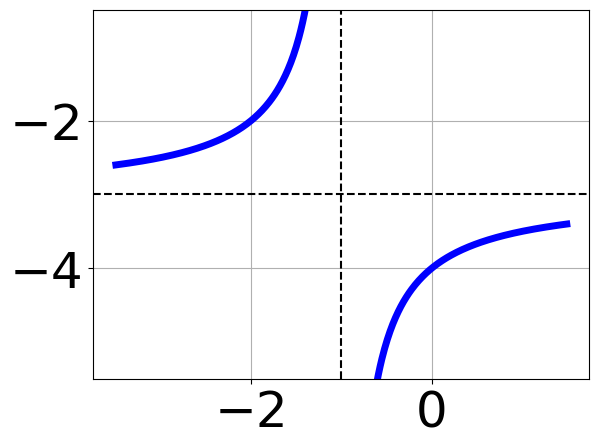
\includegraphics[width = 0.3\textwidth]{../Figures/rationalEquationToGraphAA.png}
\item 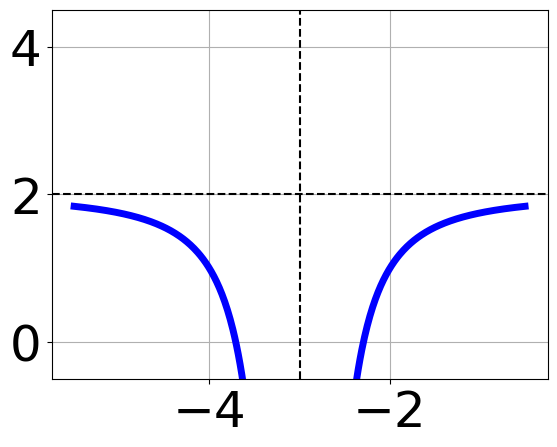
\includegraphics[width = 0.3\textwidth]{../Figures/rationalEquationToGraphBA.png}
\item 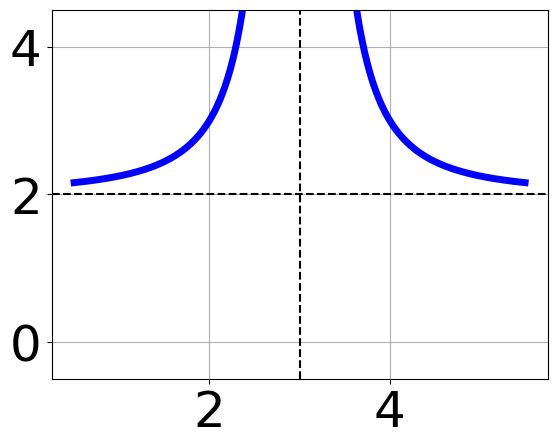
\includegraphics[width = 0.3\textwidth]{../Figures/rationalEquationToGraphCA.png}
\item 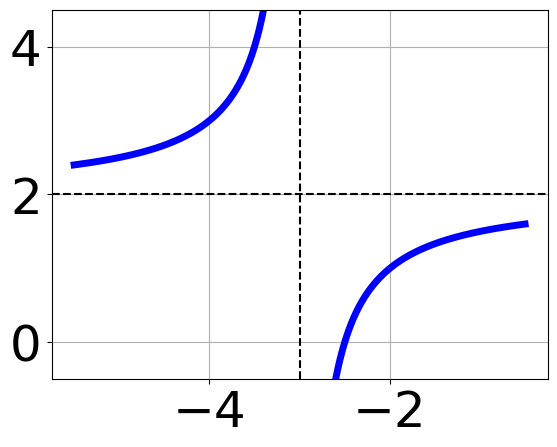
\includegraphics[width = 0.3\textwidth]{../Figures/rationalEquationToGraphDA.png}
\end{multicols}\item None of the above.\end{enumerate}
\textbf{General Comment:} Remember that the general form of a basic rational equation is $ f(x) = \frac{a}{(x-h)^n} + k$, where $a$ is the leading coefficient (and in this case, we assume is either $1$ or $-1$), $n$ is the degree (in this case, either $1$ or $2$), and $(h, k)$ is the intersection of the asymptotes.
}
\litem{
Choose the graph of the equation below.
\[ f(x) = \frac{-1}{x - 2} + 3 \]The solution is the graph below, which is option E.
\begin{center}
    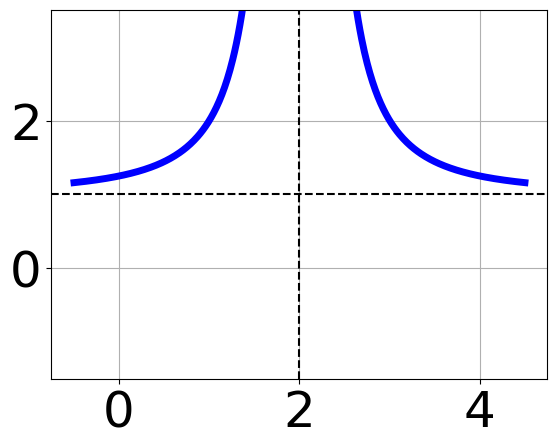
\includegraphics[width=0.3\textwidth]{../Figures/rationalEquationToGraphCopyEA.png}
\end{center}\begin{enumerate}[label=\Alph*.]
\begin{multicols}{2}
\item 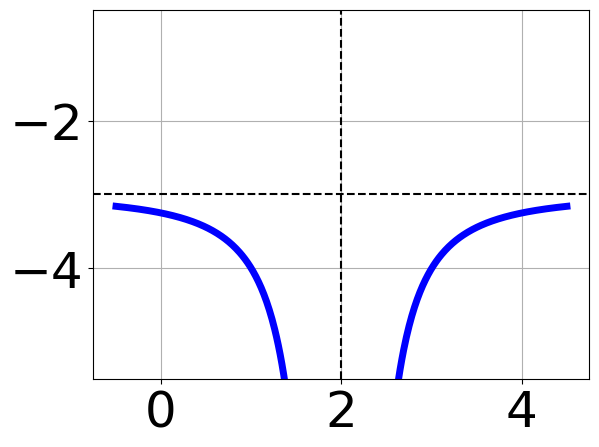
\includegraphics[width = 0.3\textwidth]{../Figures/rationalEquationToGraphCopyAA.png}
\item 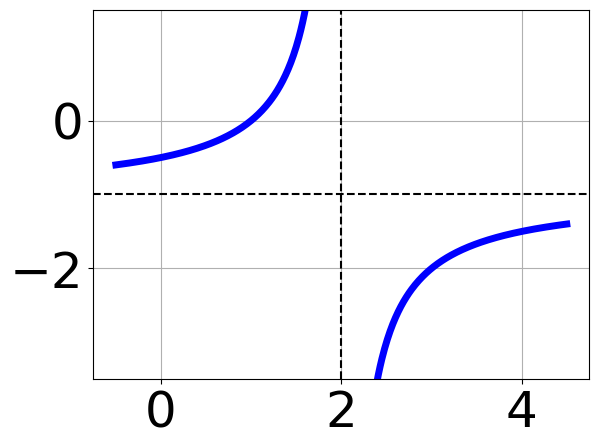
\includegraphics[width = 0.3\textwidth]{../Figures/rationalEquationToGraphCopyBA.png}
\item 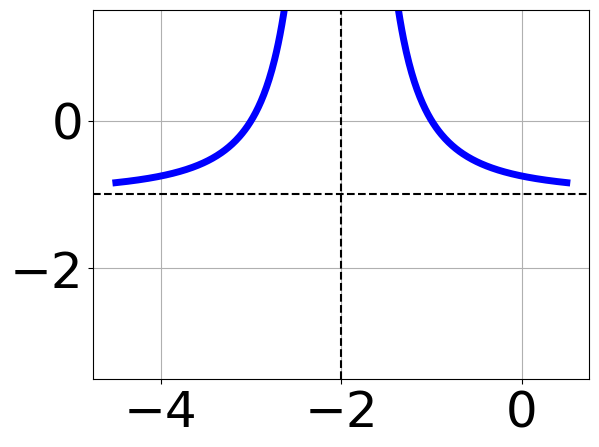
\includegraphics[width = 0.3\textwidth]{../Figures/rationalEquationToGraphCopyCA.png}
\item 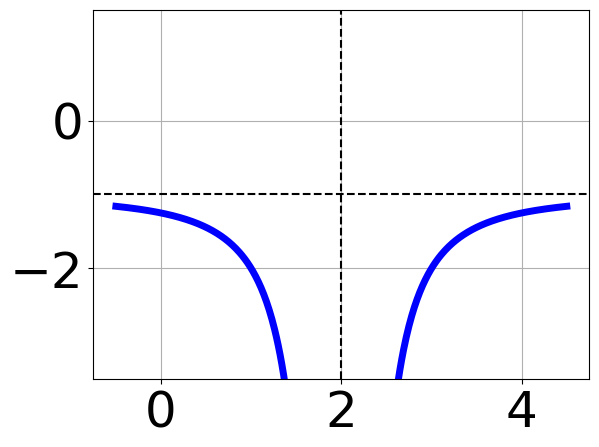
\includegraphics[width = 0.3\textwidth]{../Figures/rationalEquationToGraphCopyDA.png}
\end{multicols}\item None of the above.\end{enumerate}
\textbf{General Comment:} Remember that the general form of a basic rational equation is $ f(x) = \frac{a}{(x-h)^n} + k$, where $a$ is the leading coefficient (and in this case, we assume is either $1$ or $-1$), $n$ is the degree (in this case, either $1$ or $2$), and $(h, k)$ is the intersection of the asymptotes.
}
\litem{
Choose the equation of the function graphed below.

\begin{center}
    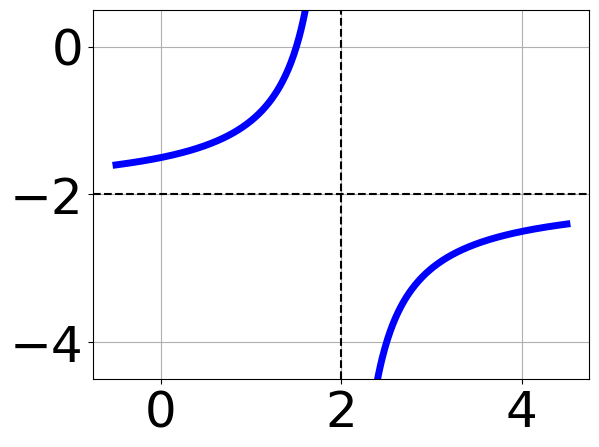
\includegraphics[width=0.5\textwidth]{../Figures/rationalGraphToEquationCopyA.png}
\end{center}


The solution is \( f(x) = \frac{-1}{x - 2} - 2 \), which is option B.\begin{enumerate}[label=\Alph*.]
\item \( f(x) = \frac{1}{(x + 2)^2} - 2 \)

Corresponds to thinking the graph was a shifted version of $\frac{1}{x^2}$, using the general form $f(x) = \frac{a}{x+h}+k$, and the opposite leading coefficient.
\item \( f(x) = \frac{-1}{x - 2} - 2 \)

This is the correct option.
\item \( f(x) = \frac{1}{x + 2} - 2 \)

Corresponds to using the general form $f(x) = \frac{a}{x+h}+k$ and the opposite leading coefficient.
\item \( f(x) = \frac{-1}{(x - 2)^2} - 2 \)

Corresponds to thinking the graph was a shifted version of $\frac{1}{x^2}$.
\item \( \text{None of the above} \)

This corresponds to believing the vertex of the graph was not correct.
\end{enumerate}

\textbf{General Comment:} Remember that the general form of a basic rational equation is $ f(x) = \frac{a}{(x-h)^n} + k$, where $a$ is the leading coefficient (and in this case, we assume is either $1$ or $-1$), $n$ is the degree (in this case, either $1$ or $2$), and $(h, k)$ is the intersection of the asymptotes.
}
\litem{
Solve the rational equation below. Then, choose the interval(s) that the solution(s) belongs to.
\[ \frac{6}{8x + 2} + -2 = \frac{-8}{-72x -18} \]The solution is \( x = 0.069 \), which is option E.\begin{enumerate}[label=\Alph*.]
\item \( \text{All solutions lead to invalid or complex values in the equation.} \)

This corresponds to thinking $x = 0.069$ leads to dividing by zero in the original equation, which it does not.
\item \( x_1 \in [-0.28, 0.41] \text{ and } x_2 \in [0.45,0.6] \)

$x = 0.069 \text{ and } x = 0.569$, which corresponds to getting the correct solution and believing there should be a second solution to the equation.
\item \( x \in [0.39,1.43] \)

$x = 0.569$, which corresponds to not distributing the factor $8x + 2$ correctly when trying to eliminate the fraction.
\item \( x_1 \in [-0.28, 0.41] \text{ and } x_2 \in [0.61,0.73] \)

$x = 0.069 \text{ and } x = 0.625$, which corresponds to getting the correct solution and believing there should be a second solution to the equation.
\item \( x \in [0.07,2.07] \)

* $x = 0.069$, which is the correct option.
\end{enumerate}

\textbf{General Comment:} Distractors are different based on the number of solutions. Remember that after solving, we need to make sure our solution does not make the original equation divide by zero!
}
\litem{
Solve the rational equation below. Then, choose the interval(s) that the solution(s) belongs to.
\[ \frac{-26}{91x + 78} + 1 = \frac{-26}{91x + 78} \]The solution is \( \text{all solutions are invalid or lead to complex values in the equation.} \), which is option D.\begin{enumerate}[label=\Alph*.]
\item \( x \in [-0.14,1.86] \)

$x = 0.857$, which corresponds to not distributing the factor $91x + 78$ correctly when trying to eliminate the fraction.
\item \( x \in [-1.86,0.14] \)

$x = -0.857$, which corresponds to not checking if this value leads to dividing by 0 in the original equation and thus is not a valid solution.
\item \( x_1 \in [-3.86, 0.14] \text{ and } x_2 \in [-0.4,1] \)

$x = -0.857 \text{ and } x = 0.857$, which corresponds to getting the correct solution and believing there should be a second solution to the equation.
\item \( \text{All solutions lead to invalid or complex values in the equation.} \)

*$x = -0.857$ leads to dividing by 0 in the original equation and thus is not a valid solution, which is the correct option.
\item \( x_1 \in [-3.86, 0.14] \text{ and } x_2 \in [-1.8,0.1] \)

$x = -0.857 \text{ and } x = -0.857$, which corresponds to getting the correct solution and believing there should be a second solution to the equation.
\end{enumerate}

\textbf{General Comment:} Distractors are different based on the number of solutions. Remember that after solving, we need to make sure our solution does not make the original equation divide by zero!
}
\litem{
Solve the rational equation below. Then, choose the interval(s) that the solution(s) belongs to.
\[ \frac{-4x}{3x + 5} + \frac{-6x^{2}}{-9x^{2} -33 x -30} = \frac{2}{-3x -6} \]The solution is \( \text{There are two solutions: } x = 0.479 \text{ and } x = -3.479 \), which is option D.\begin{enumerate}[label=\Alph*.]
\item \( x_1 \in [-0.23, 0.72] \text{ and } x_2 \in [-2.67,0.33] \)


\item \( x \in [-5.8,-2.34] \)


\item \( \text{All solutions lead to invalid or complex values in the equation.} \)


\item \( x_1 \in [-0.23, 0.72] \text{ and } x_2 \in [-5.48,-2.48] \)

* $x = 0.479 \text{ and } x = -3.479$, which is the correct option.
\item \( x \in [-2.32,-1.28] \)


\end{enumerate}

\textbf{General Comment:} Distractors are different based on the number of solutions. Remember that after solving, we need to make sure our solution does not make the original equation divide by zero!
}
\litem{
Choose the equation of the function graphed below.

\begin{center}
    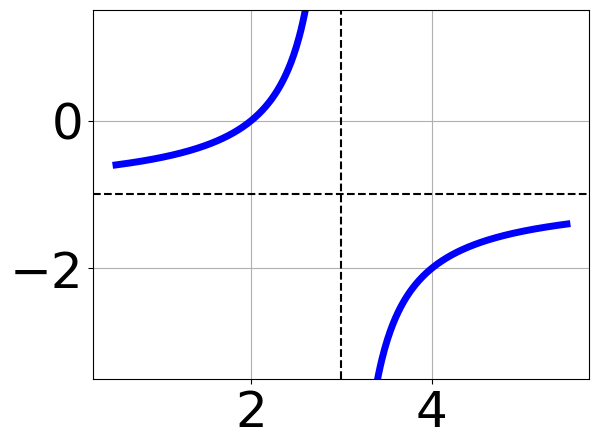
\includegraphics[width=0.5\textwidth]{../Figures/rationalGraphToEquationA.png}
\end{center}


The solution is \( \text{None of the above as it should be } f(x) = \frac{-1}{x - 3} - 1 \), which is option E.\begin{enumerate}[label=\Alph*.]
\item \( f(x) = \frac{1}{x + 3} - 2 \)

Corresponds to using the general form $f(x) = \frac{a}{x+h}+k$, the opposite leading coefficient AND not noticing the $y$-value was wrong.
\item \( f(x) = \frac{-1}{x - 3} - 2 \)

The $y$-value of the equation does not match the graph.
\item \( f(x) = \frac{-1}{(x - 3)^2} - 2 \)

Corresponds to thinking the graph was a shifted version of $\frac{1}{x^2}$ not noticing the $y$-value was wrong.
\item \( f(x) = \frac{1}{(x + 3)^2} - 2 \)

Corresponds to thinking the graph was a shifted version of $\frac{1}{x^2}$, using the general form $f(x) = \frac{a}{x+h}+k$, the opposite leading coefficient, AND not noticing the $y$-value was wrong.
\item \( \text{None of the above} \)

None of the equation options were the correct equation.
\end{enumerate}

\textbf{General Comment:} Remember that the general form of a basic rational equation is $ f(x) = \frac{a}{(x-h)^n} + k$, where $a$ is the leading coefficient (and in this case, we assume is either $1$ or $-1$), $n$ is the degree (in this case, either $1$ or $2$), and $(h, k)$ is the intersection of the asymptotes.
}
\end{enumerate}

\end{document}